\documentclass[utf8x,xcolor=pdftex,dvipsnames,table]{beamer}
\usetheme{Malmoe}  % Now it's a beamer presentation with the lisa theme!
\setbeamertemplate{footline}[page number]
\usecolortheme{beaver}
\usepackage[T1]{fontenc}
\usepackage{amsmath}
\usepackage[utf8x]{inputenc}
\logo{\includegraphics[width=.8in]{UdeM_NoirBleu_logo_Marie_crop.pdf}}

\mode<presentation>

\title{A Common GPU n-Dimensional Array for Python and C}

\author{
\footnotesize
Frédéric Bastien, Arnaud Bergeron, Pascal Vincent and Yoshua Bengio \newline
Département d'Informatique et de Recherche Opérationnelle \newline
Université de Montréal \newline
Montréal, Canada \newline
\texttt{\{bastienf, bergearn, vincentp, bengioy\}@iro.umontreal.ca}
}

\date{NIPS 2011 Big Learning Workshop}

\setbeamertemplate{navigation symbols}{}

\begin{document}

\begin{frame}[plain]
 \titlepage
 
\includegraphics[width=1in]{lisabook_logo_text_3.png}
 \hfill
 \includegraphics[width=.8in]{UdeM_NoirBleu_logo_Marie_crop.pdf}
\end{frame}
\addtocounter{framenumber}{-1}

%\begin{frame}{Outline}
% \tableofcontents
%\end{frame}

\section{Motivation}

\begin{frame}{Why do we need this?}
\begin{itemize}
\item Efficient linear algebra is a the core of many scientific applications
\item On the CPU, numpy provides a standard object (for python at least)
\end{itemize}
\end{frame}

\begin{frame}{Why a new implementation?}
\begin{block}{There are already a number of existing GPU computing codebases:}
Theano, PyCUDA/PyOpenCL, CUDAmat, Gnumpy, Thrust, ...
\end {block}
\begin{enumerate}
\item<2-> All are incompatible
\item<3-> They do not support the full range of numpy features
\item<4-> None support both CUDA and OpenCL
\end{enumerate}
\end{frame}

\section{Features}
\begin{frame}{Features desired}
\begin{itemize}
\item Support for varying datatypes
\item Support for an arbitrary number of dimensions
\item Support for strides
\item Support for broadcasting
\item Compatibility with CUDA and OpenCL
\end{itemize}
\end{frame}

\begin{frame}{Strides}
\begin{center}
\onslide<1->{Matrix ${\color{red!50}A}$}\hspace{5em}\onslide<2->{Matrix ${\color{cyan!50}B}$}
\end{center}
\begin{center}
\only<1>{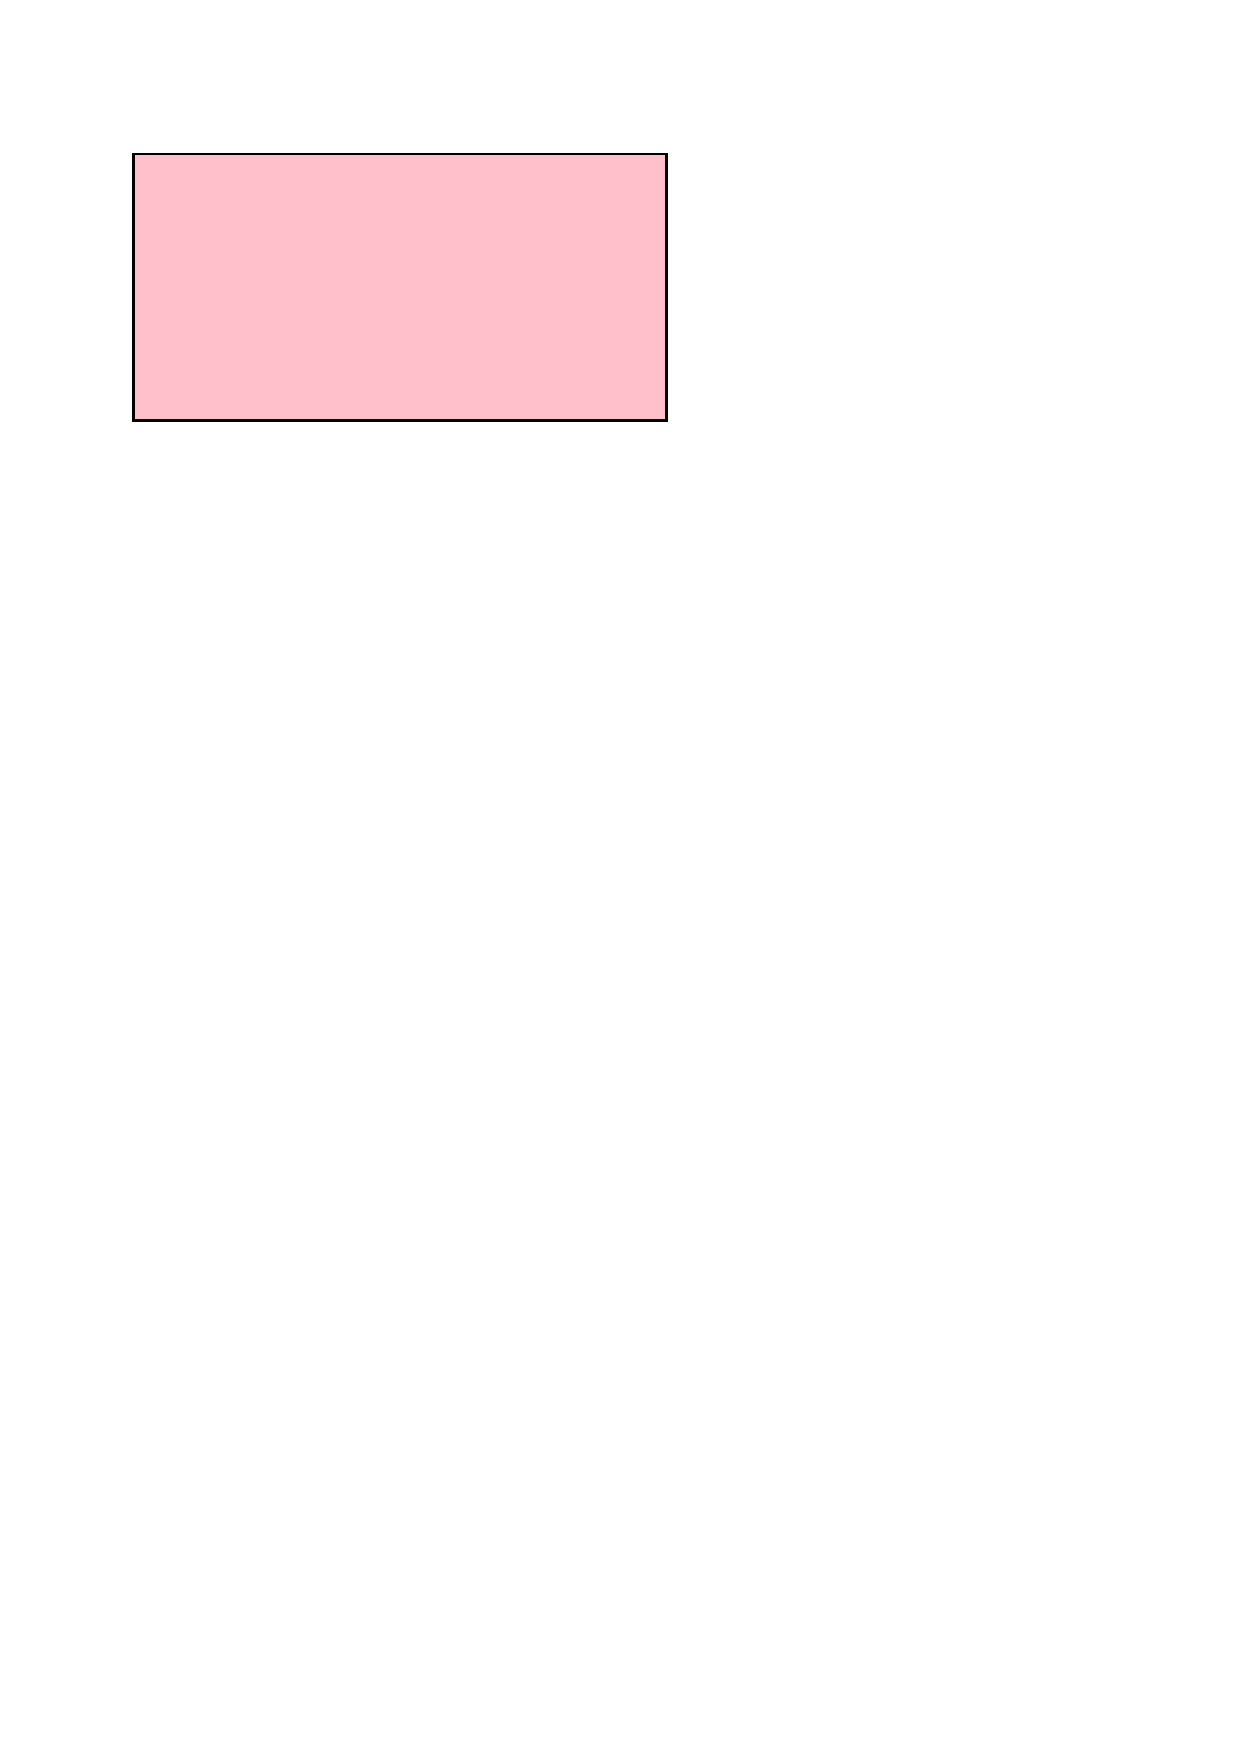
\includegraphics{strides-1}}
\only<2>{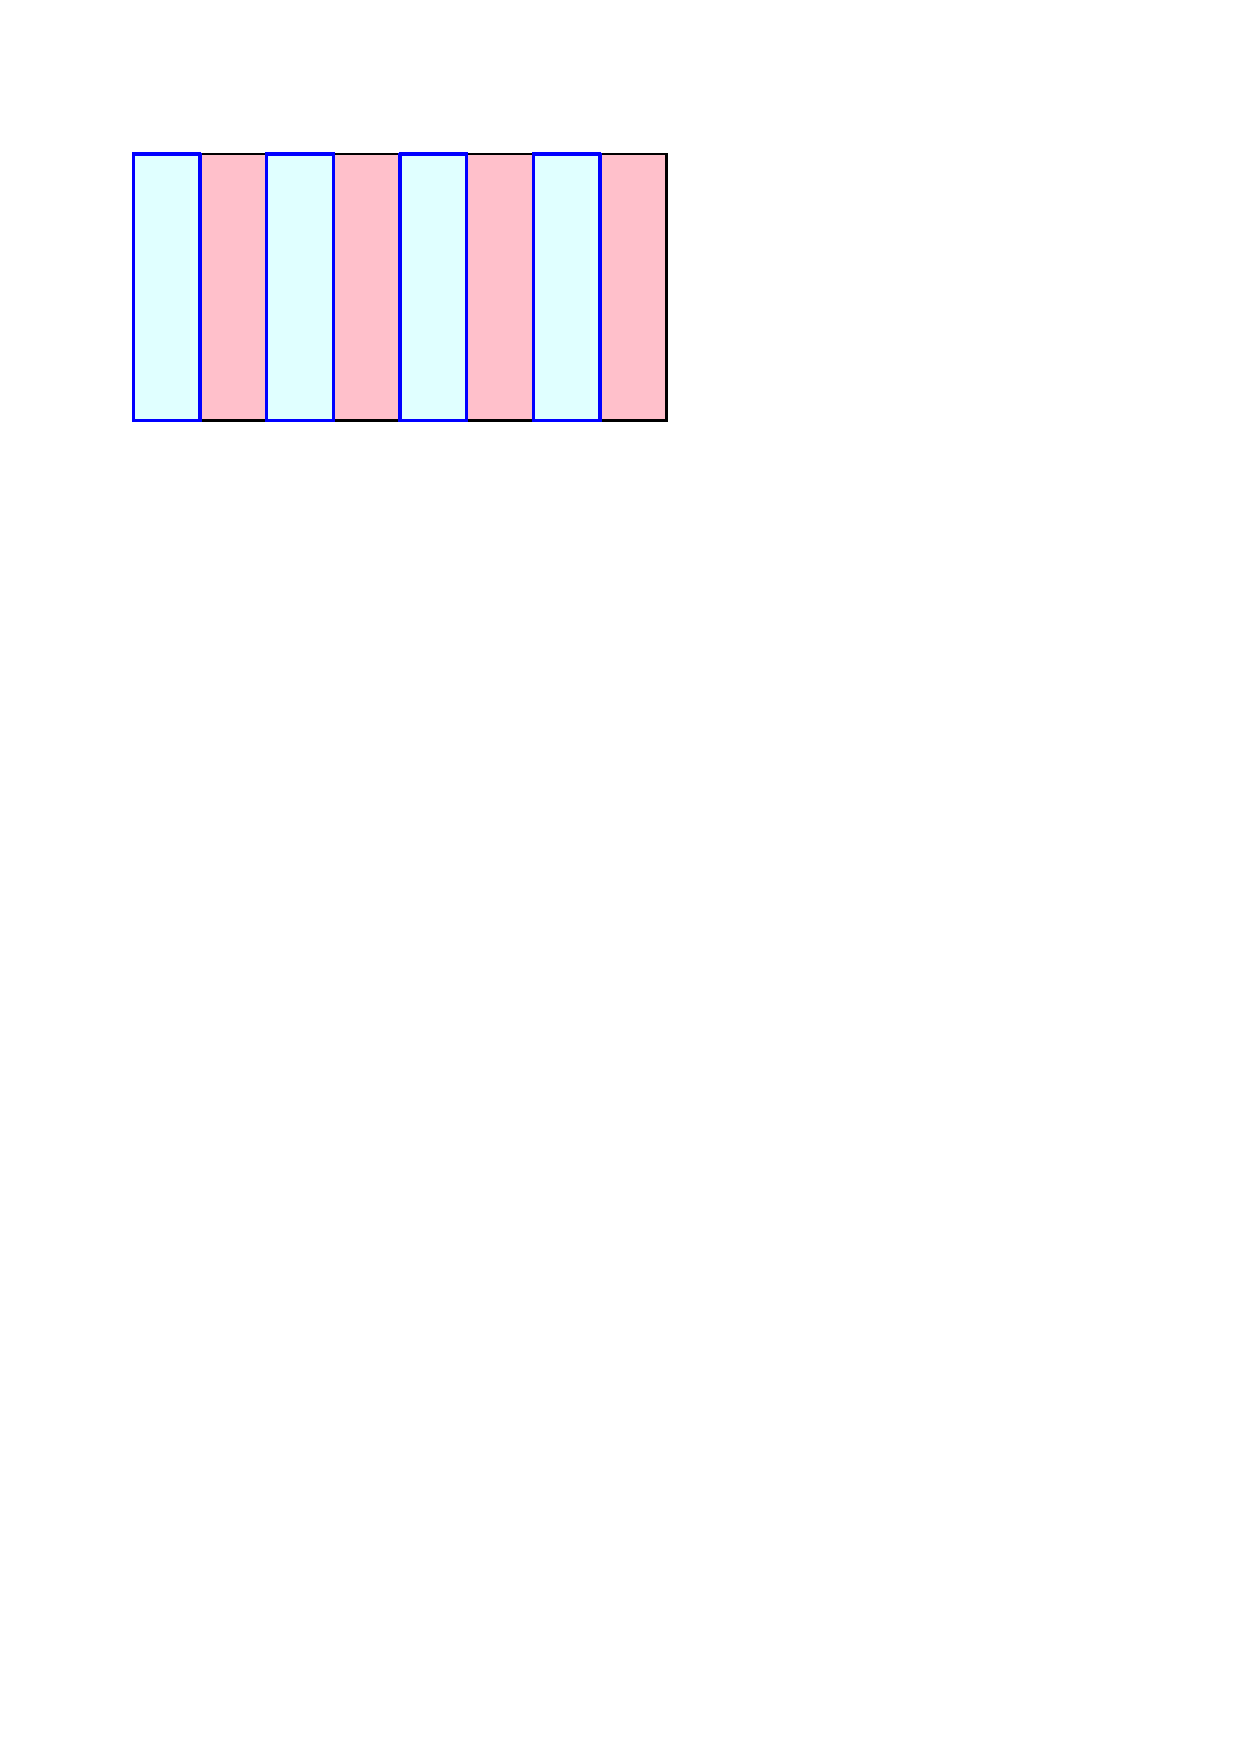
\includegraphics{strides-2}}
\end{center}
\only<1>{If we do something like ${\color{cyan!50}B} = {\color{red!50}A}$\texttt{[:,::}2\texttt{]},}
\only<2>{we get the matrix ${\color{cyan!50}B}$ that shares memory with ${\color{red!50}A}$.}
\end{frame}

\begin{frame}{Broadcasting}
\only<1>{We have matrix ${\color{red!50}A}$ of size (8,8) and we want to multiply it by vector ${\color{cyan!50}B}$ of size (8,1).}
\only<2>{So we make virtual copies of ${\color{cyan!50}B}$ along the last dimension until it has the same size as ${\color{red!50}A}$.}
\begin{center}
\only<1>{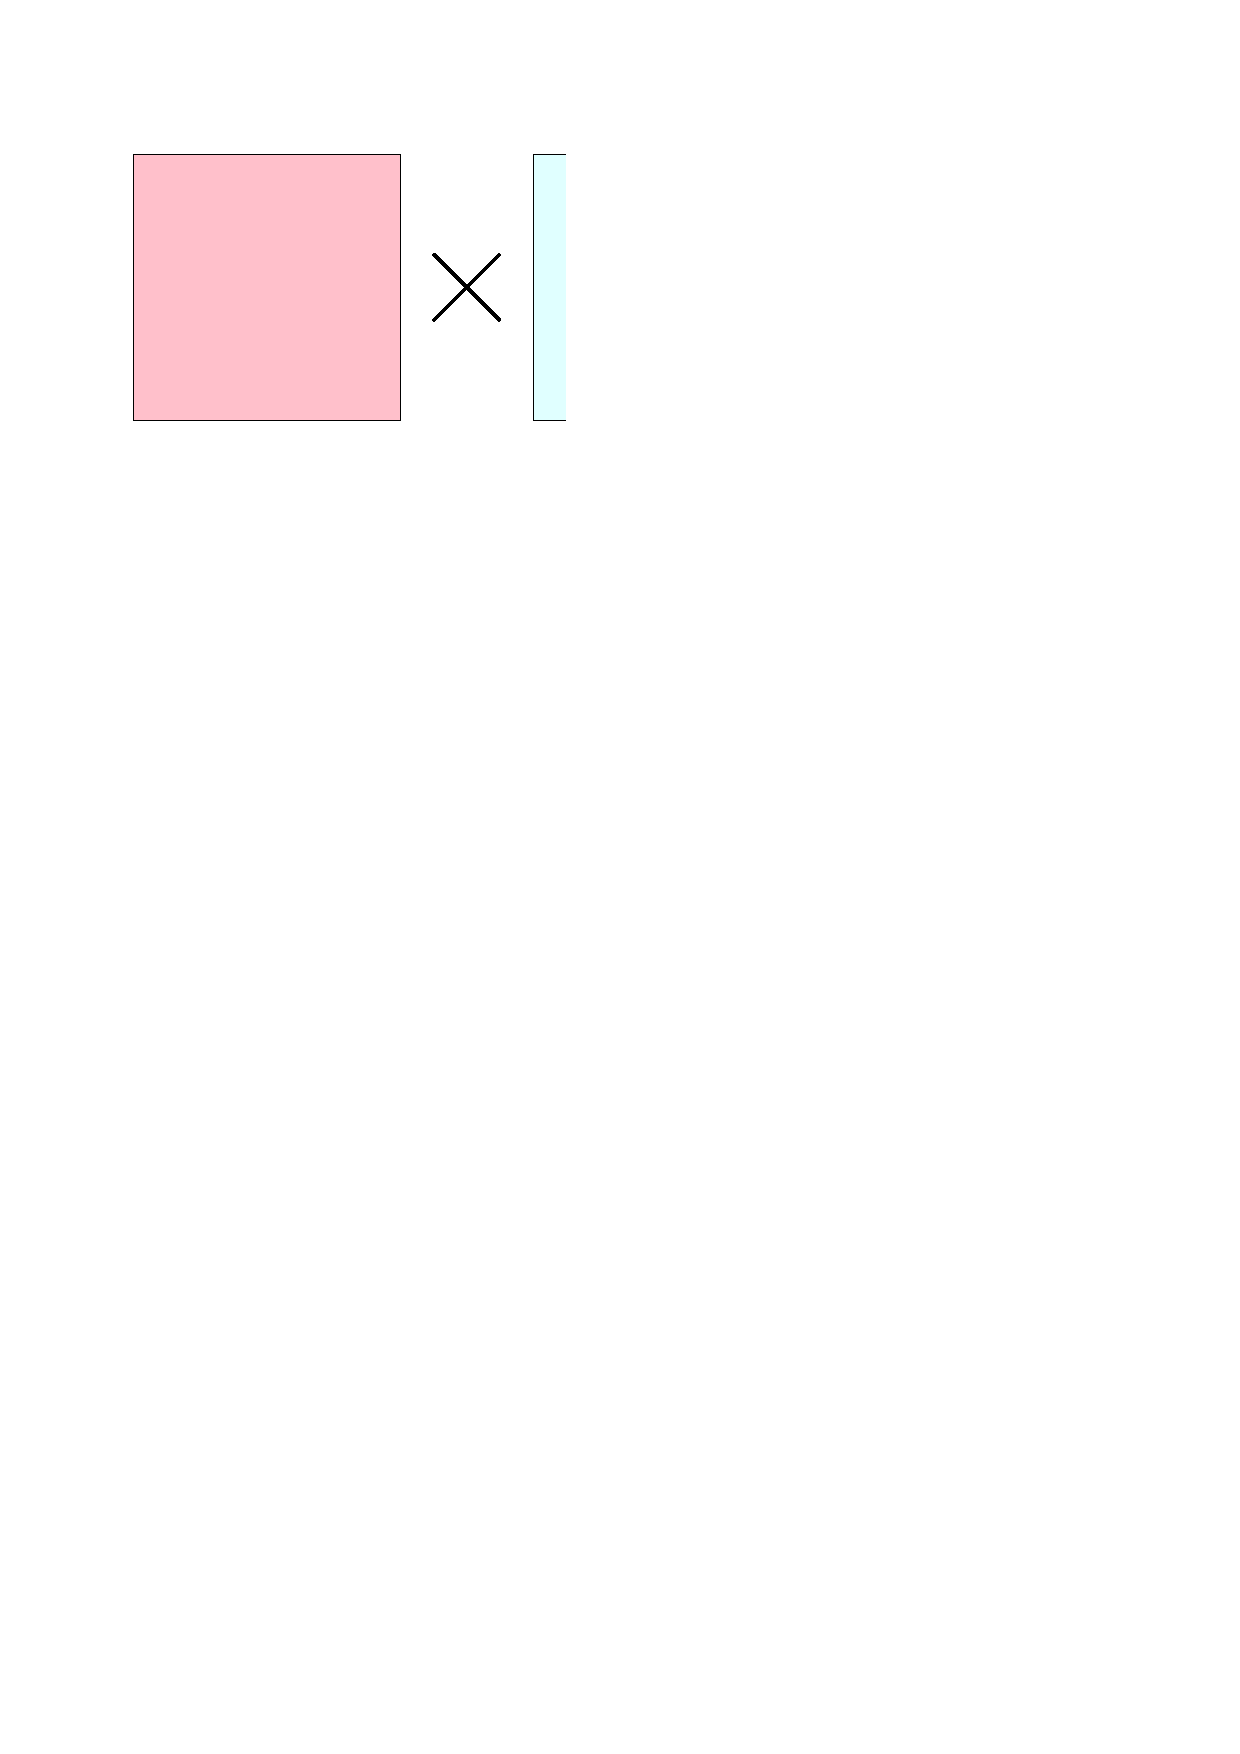
\includegraphics[width=0.9\textwidth]{bcast-1}}
\only<2>{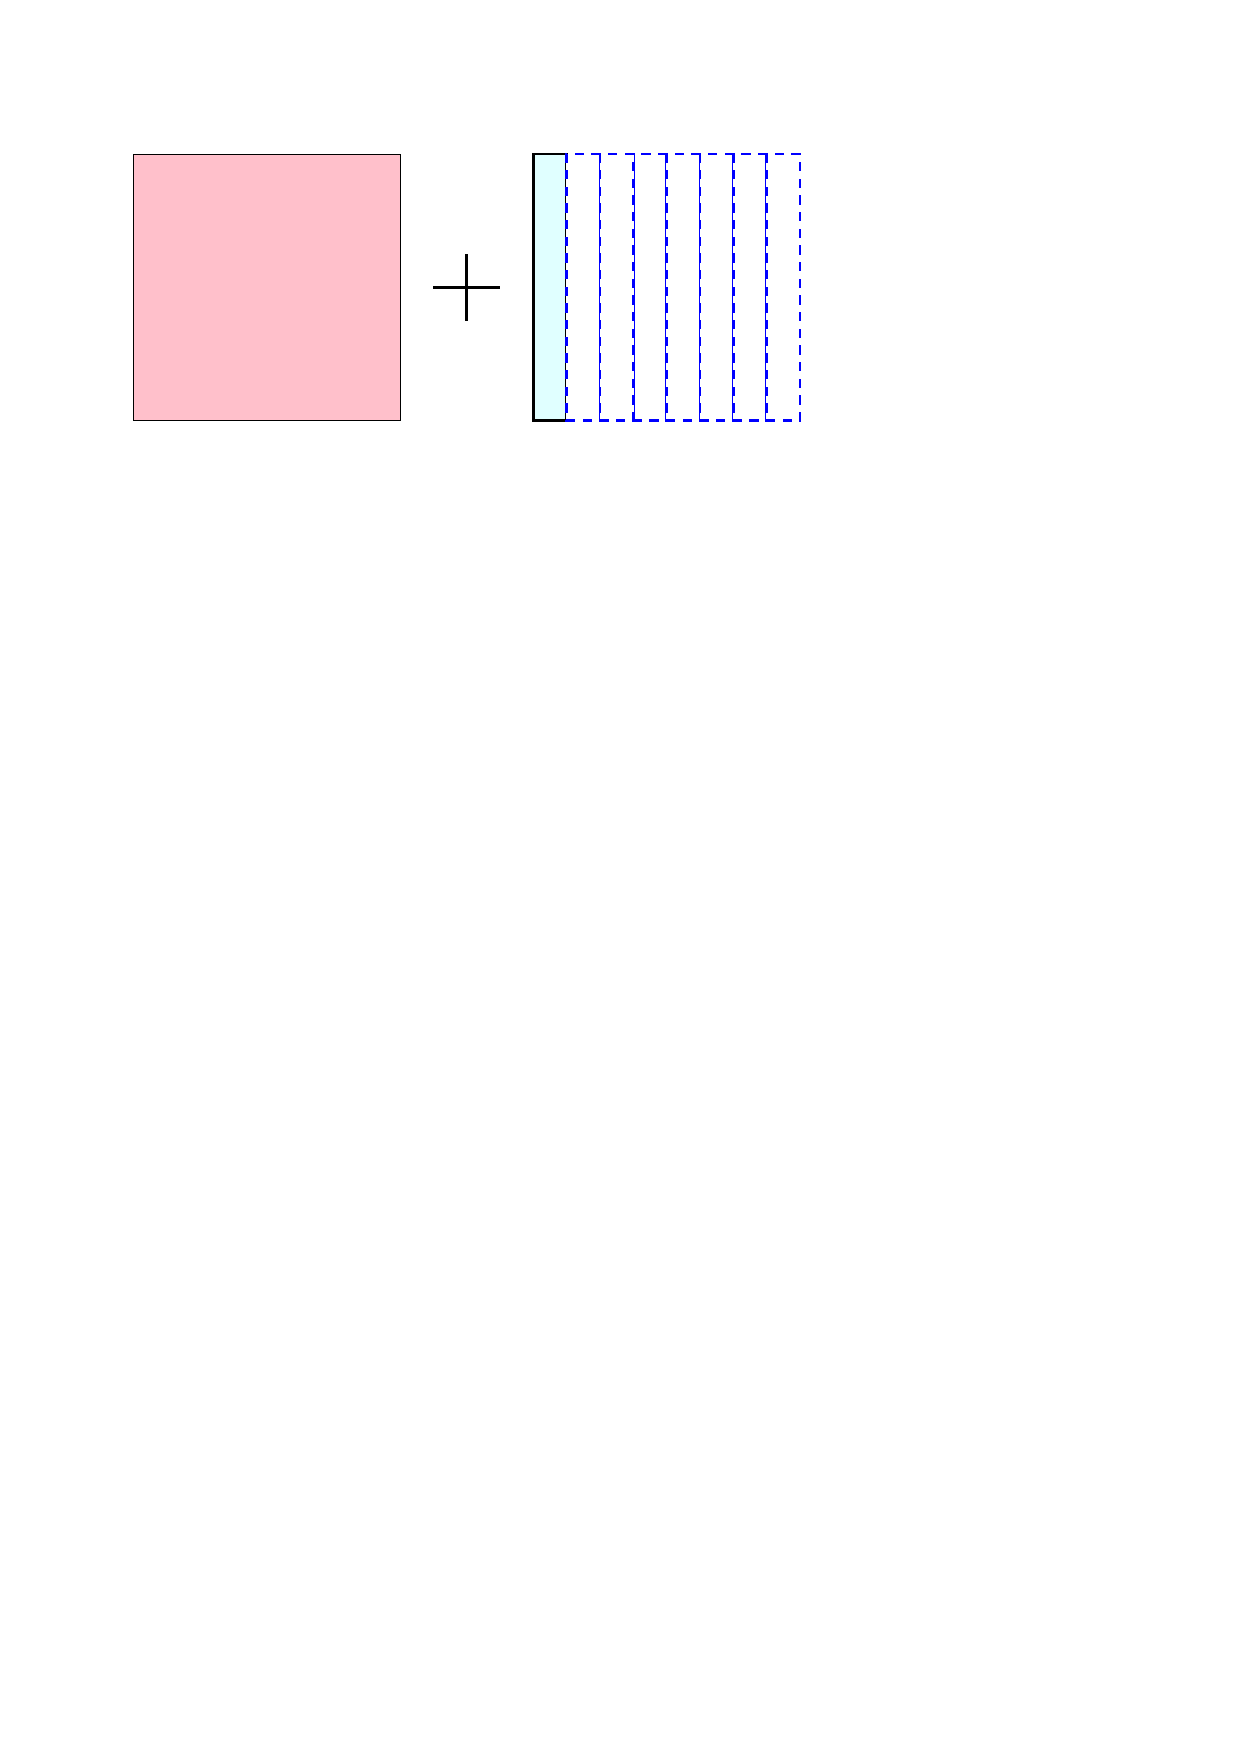
\includegraphics[width=0.9\textwidth]{bcast-2}}
\end{center}
\only<1>{This doesn't fit the rules for elementwise operations since both objects do not have the same number of elements.}
\only<2>{Then we can proceed as usual.  Fixing things this way is often a very useful tool when doing some computations.}
\end{frame}

\begin{frame}{Why has this not been done before?}
\begin{itemize}
\item Hard and time consuming to get right and efficent
\item Certain algorithms cannot work on a general memory layout
\item Indexing computations take up a significant portion of time on the GPU
\end{itemize}
\end{frame}

\begin{frame}{Easy to develop}
\begin{itemize}
\item Not always a good idea to make a gpu code work for all memory layout.
  \begin{itemize}
  \item Harder to code
  \item Harder to get efficient
  \end{itemize}
\item Just call \begin{bf}as\_\{contiguous,fortran\}\_memory()\end{bf}
 on inputs!
\end{itemize}
\end{frame}

\section{Exisiting Implementations}

\begin{frame}{Comparison of existing implementations}
\begin{table}
\rowcolors{2}{RoyalBlue!5}{RoyalBlue!23}
\begin{tabular}{|l|c|c|c|c|c|}
\hline
Package & strides & bcast & dims & types & backends \\
\hline
\hline
Theano & yes\footnote{as number of elements} & yes & any & float32 & CUDA \\
PyCUDA& no & no & any & all & CUDA \\
PyOpenCL & no & no & any & all & OpenCL \\
CUDAMat & no & yes\footnote{via a function} & 2 & float32 & CUDA \\
Gnumpy & no & yes & any & float32\footnote{and a hackish form of boolean} & CUDA \\
Thrust & no & no & 1 & all & CUDA \\
\hline
\hiderowcolors
Desired & yes & yes & any & all & both \\
\hline
\end{tabular}
\end{table}
\end{frame}

\section{Current State}

\begin{frame}{Functionality}
\begin{block}{What we have}
\begin{itemize}
\item all the feature wanted: strides, bcast, dims, types, backends
\item allocation, transfer
\item views
\item elementwise kernels
\item partial reductions
\item support for CUDA and OpenCL
\end{itemize}
\end{block}
\begin{block}{Interface}
\begin{itemize}
\item Python
\item C++ interface similar to Numpy C-API
\end{itemize}
\end{block}
\end{frame}

\begin{frame}{Missing Functionality}
\begin{block}{What we miss}
\begin{itemize}
\item assignation
\item reshaping
\end{itemize}
\end{block}
\end{frame}

\subsection{Element-wise dimension collapsing}
% pretty pictures would be better
\begin{frame}{Dimension collapsing}
\begin{itemize}
\item Computing indexes takes time
\item On contiguous memory n-d and 1-d are the same for element-wise operations
\item So we can merge all dimensions into one for the kernel
\item When dimensions are not all contiguous we can still merge adjacent contiguous ones
\end{itemize}
\end{frame}

\section{Benchmarks}
\begin{frame}{Benchmarks}
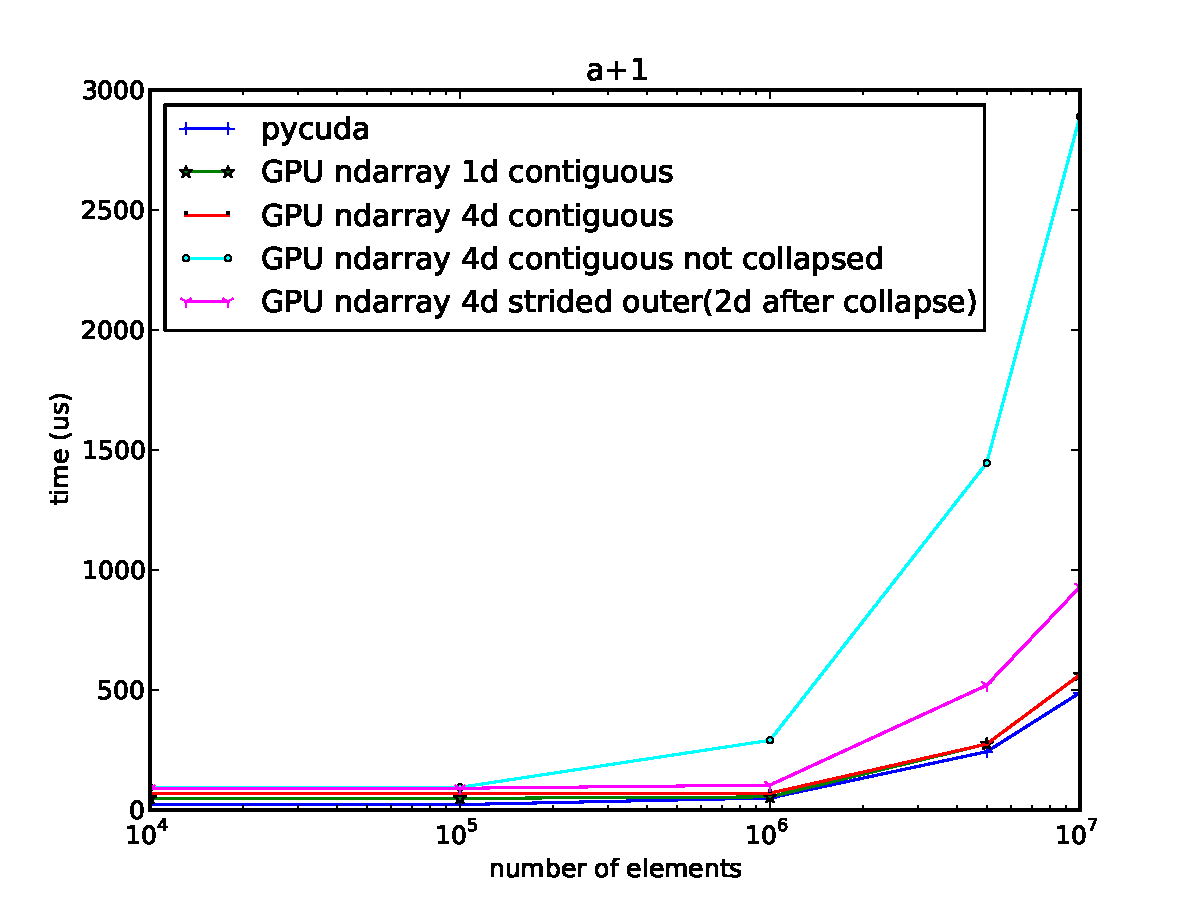
\includegraphics[width=\textwidth]{ap1_no_alloc}
\end{frame}

\begin{frame}{Benchmarks (cont.)}
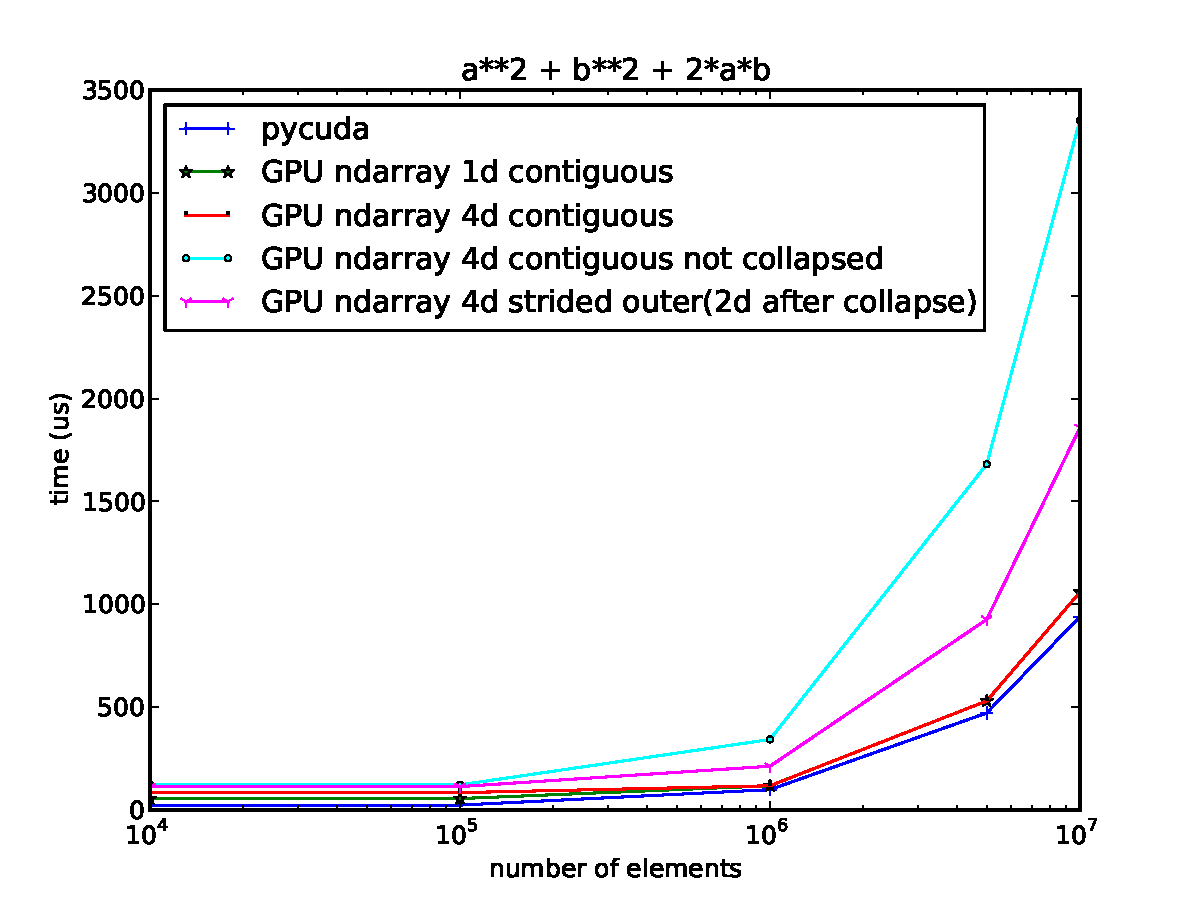
\includegraphics[width=\textwidth]{a2pb2p2ab_no_alloc}
\end{frame}

\section{Future Plans}
\begin{frame}{Future plans}
\begin{itemize}
\item<1-> Design and implement a good C/C++ interface
\item<2-> Find ways to lower the overhead
\item<3-> Use the implicit looping provided by CUDA and OpenCL
\item<4-> World domination!
\item<5-> ???
\item<6-> Profit
\end{itemize}
\end{frame}

\section*{Questions}
\begin{frame}
\begin{center}
\Huge
Questions?
\end{center}
\end{frame}


\end{document}
